\section{結果}
\label{sec_results}
\subsection{属性の頻度と再現性}
全データの推定では，場面の文字は35.0\%，吹き出しは14.3\%，重ねた文字は8.3\%，余白の文字は12.1\%の画像にあり，いずれかの層がある画像は58.7\%であった．
この割合は，パッケージが文字ありとした代表の画像の割合と一致する．
付け直した90枚では，層と形の記号の完全一致は94.4\%であった．
層ごとの $ \kappa $ は0.95〜1.00であり，規則で導いたお題文ありの $ \kappa $ は $ r_{1b} $ で1.00，$ r_1 $ で0.97，$ r_2 $ で0.92であった．
不一致は，小さな場面の文字の見落とし，テレビの字幕の層の判断，名札や曲名をその他の文として記録するかの判断にあった．

\subsection{規則とお題文ありの割合}
表\ref{tab_shift}に，規則ごとに導いたお題文ありと，第5版の目視のお題文ありとの一致を示す．
v5 のみと v6 のみは，それぞれ一方の定義でのみお題文ありとなる画像の割合である．

\begin{table}[t]
    \centering
    \caption{規則で導いたお題文ありと第5版の目視ラベルとの一致（全データの推定）．第5版のお題文ありの割合は7.93\%である}
    \label{tab_shift}
    \small
    \begin{tabular}{cccccc}
        \toprule
        規則 & 一致率 & $ \kappa $ & 割合 & v5 のみ & v6 のみ \\
        \midrule
        $ r_0 $ & 98.1\% & 0.864 & 7.40\% & 1.23\% & 0.70\% \\
        $ r_1 $ & 97.3\% & 0.839 & 10.31\% & 0.15\% & 2.52\% \\
        $ r_{1b} $ & 98.5\% & 0.904 & 8.95\% & 0.23\% & 1.26\% \\
        $ r_{1b}' $ & 98.6\% & 0.906 & 8.31\% & 0.52\% & 0.89\% \\
        $ r_2 $ & 91.1\% & 0.592 & 16.67\% & 0.10\% & 8.84\% \\
        \bottomrule
    \end{tabular}
\end{table}

規則を変えるだけで，お題文ありの割合は7.40\%から16.67\%まで変わった．
$ r_{1b} $ は第5版と最もよく一致し，$ \kappa $ は0.904であった．
$ r_2 $ は第5版から大きく離れ，お題文ありの割合が約2倍になった．
重ねた文字の台詞や字幕は，第5版では多くがお題文なしであったためである．

1,620枚で $ r_1 $ と $ r_{1b} $ の判定が分かれた画像は34枚であり，いずれも余白に空欄を含む文とその他の文がある画像であった．
そのうち24枚は第5版でお題文なしであり，キャラクターの紹介の画面の名前，「なぞかけ」の名札，映画の題名などであった．
残りの10枚は第5版でお題文ありであり，空欄の文とは別に置いた状況の文や見出しの画像であった．

重ねた文字に問い，指示，題目の句がある画像は，1,620枚で53枚であった．
そのうち第5版でお題文ありは18枚，お題文なしは35枚であり，お題文なしの35枚の多くは，アニメや映画の台詞の字幕が問いの形になったものであった．
全データの推定では，これらの画像は全体の0.65\%であり，第5版でお題文ありが0.28\%，お題文なしが0.37\%であった．
$ r_{1b} $ と $ r_{1b}' $ の第5版との $ \kappa $ は0.904と0.906であり，重ねた文字の問いを含めるかは，第5版との一致ではほぼ決まらない．

\subsection{教師と生徒の属性の精度}
図\ref{fig_attrs}に，1,620枚での属性ごとの F1 を示す．
横軸は属性であり，左の4項目が層，右の10項目が層ごとの文の形である．
括弧内は正例の数である．
縦軸は目視ラベルに対する F1 である．

教師の層の F1 は0.57〜0.76であり，いずれの層でも再現率が0.87以上，適合率が0.64以下であった．
教師は層を広く真と答え，場面の文字を真とした誤り651枚のうち370枚は文字の層がない画像，余白の文字の誤り355枚のうち235枚はスクリーンショットや看板などの場面の文字の画像であった．
層をまとめた文の形の F1 は，問い0.78，空欄を含む文0.77，指示0.73，題目の句0.71，その他の文0.55であり，教師は文字がどこにあるかよりも，どの形の文があるかを答える方が得意であった．

生徒は，余白の文字と吹き出しを埋め込みだけでいずれも F1 0.85 で学べ，教師を上回った．
一方，場面の文字は0.67，重ねた文字は0.62にとどまった．
文の形は，余白の空欄を含む文が0.72であったほかは，埋め込みだけでは0.0〜0.54であった．
文の特徴を加えると多くの形で F1 が上がったが，重ねた文字の問い，指示，題目の句は正例が5〜38枚と少なく，ほとんど学べなかった．
教師の書き起こしを YomiToku の書き起こしに替えても，形の F1 の差は小さかった．

\subsection{導いたお題文ありの精度}
表\ref{tab_odai}に，$ r_{1b} $ で導いた目視のお題文ありを正解としたときの，各方法のお題文ありの F1 を示す．
参考として，第5版の目視のお題文ありを正解とした値を併記する．

\begin{table}[t]
    \centering
    \caption{お題文ありの F1（全データの推定）．括弧は95\%区間}
    \label{tab_odai}
    \footnotesize
    \setlength{\tabcolsep}{2pt}
    \begin{tabular}{lcc}
        \toprule
        方法 & 正解 $ r_{1b} $ & 正解 第5版 \\
        \midrule
        パッケージ v5.3.0 & 0.828 [0.79, 0.86] & 0.829 \\
        教師の属性から導く & 0.434 [0.36, 0.53] & 0.398 \\
        生徒の属性：埋め込み & 0.650 [0.55, 0.76] & 0.653 \\
        生徒の属性：＋文（32B） & 0.730 [0.64, 0.83] & 0.732 \\
        生徒の属性：＋文（YomiToku） & 0.773 [0.70, 0.84] & 0.783 \\
        直接学習：埋め込み & 0.751 [0.63, 0.86] & 0.733 \\
        直接学習：＋文（32B） & 0.785 [0.67, 0.89] & 0.755 \\
        \bottomrule
    \end{tabular}
\end{table}

教師の属性から導いたお題文ありは，F1 が0.434にとどまった．
層の誤りが規則に伝わり，お題文ありを広く真としたためである．
1,620枚で学習した生徒は，いずれもパッケージ v5.3.0 に届かなかった．
属性を経る生徒では，埋め込みに YomiToku の書き起こしを加えた場合が最も高く，F1 は0.773であった．
パッケージ v5.3.0 は，正解を $ r_{1b} $ としても第5版としても F1 が約0.83 であり，$ r_{1b} $ の定義が第5版に近いことを示している．

図\ref{fig_curve}に，学習に用いた画像の数と分割外の F1 の関係を示す．
横軸は5分割のうち学習に用いた画像の数であり，縦軸は1,620枚の重みなしの F1 である．
余白の文字は約300枚で F1 0.8 に達した．
一方，直接学習したお題文ありは約650枚以降で伸びが小さく，問いとその他の文は1,296枚でも0.5前後であった．

\begin{figure}[t]
    \centering
    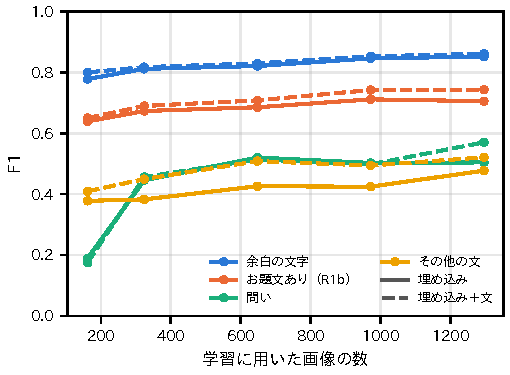
\includegraphics[width=\columnwidth]{figures/fig_curve.pdf}
    \caption{学習に用いた画像の数と分割外の F1．実線は埋め込みのみ，破線は埋め込みと教師の書き起こしの文を入力とした生徒である}
    \label{fig_curve}
\end{figure}

\subsection{書き起こしの費用}
表\ref{tab_speed}に，1,620枚での書き起こしと属性の問い合わせの速さと，パッケージが文字ありとした代表の画像の全てに適用した場合の見積もりを示す．
いずれも単一の GPU での値である．

\begin{table}[t]
    \centering
    \caption{書き起こしの速さと，文字ありの代表の画像約388万枚への適用の見積もり}
    \label{tab_speed}
    \small
    \begin{tabular}{lcc}
        \toprule
        方法 & 枚/秒 & 見積もり \\
        \midrule
        32B，属性と書き起こし & 2.7 & 約16.8日 \\
        32B，書き起こしのみ & 7.5 & 約6.0日 \\
        2B，書き起こしのみ & 21.2 & 約2.1日 \\
        YomiToku & 6.2 & 約7.2日 \\
        \bottomrule
    \end{tabular}
\end{table}
